\documentclass{beamer}

% Theme and page layout
\usetheme{gapz}
\setbeamertemplate{navigation symbols}{}

% Fonts
\usepackage{fontspec}
\defaultfontfeatures{Mapping=tex-text,Scale=MatchLowercase,Numbers=Lining}
%\setsansfont[
%	ItalicFont = Whitney MediumItalic,
%	BoldFont = Whitney Semibold,
%	BoldItalicFont = Whitney SemiboldItalic,
%	SmallCapsFont = Whitney MediumSC
%]{Whitney Medium}

% Language
\usepackage{polyglossia}
\setdefaultlanguage{english}

% Graphics
\usepackage{graphicx}
\graphicspath{{./images/}}
\usepackage{multicol}

\title{Three-dimensional modeling and printing project}
\subtitle{Third-year project}
\author[V. Duvert, A. Lubineau, C. Naud, J. Packer, F. Ribon]{\scriptsize
Vincent~Duvert \\ Antoine~Lubineau \\ Caroline~Naud \\ James~Packer \\ Florian~Ribon}
\date{from January 23 to March 16, 2012}

\titlegraphic{
\includegraphics[width=4cm]{inp-enseeiht}}

\begin{document}

\frame{\titlepage}

\section{Presentation of the project}

\subsection{Clients}
\begin{frame}
	\frametitle{}
	
	\begin{block}{The \textsc{VORTEX} team of IRIT}
		\begin{itemize}
		\item \textsc{IRIT} : a research institute in computer science from Toulouse
		\item \textsc{VORTEX} : Visual Objects : from Reality To EXpression
		\item skills in the areas of graphic computing,  computer vision, artificial intelligence and networks
		\item recently acquired an uncalibrated Ultimaker 3D printer
		\item recently acquired an Ultimaker 3D printer that it can not actually use
		\end{itemize}
    \end{block}
    
    \begin{center}
		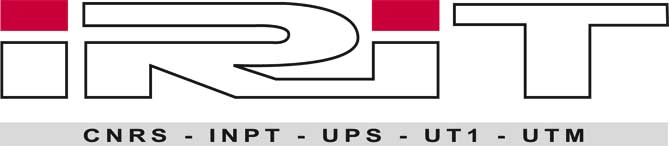
\includegraphics[width=4cm]{irit}
	\end{center}
    
\end{frame}

\subsection{Resources}
\begin{frame}
	\frametitle{}
	
	\begin{block}{The project team}
		\begin{itemize}
		\item Five final year students at ENSEEIHT, Computing and Applied Mathematics department
		\item Several followed the “multimedia” option in third year
		\item Project manager : Caroline \textsc{Naud}
		\end{itemize}
    \end{block}
    
    \begin{block}{The material resources}
    	\begin{itemize}
		\item Room F117 in building F at ENSEEIHT
    	\item Ultimaker 3D printer with a roll of PLA plastic
    	\item Computer with dual-touch screen Acer T231H
    	\item Computer rooms of the ENSEEIHT and personal computers
		\end{itemize}
    \end{block}
      
\end{frame}

\begin{frame}
	\frametitle{Ultimaker 3D printer}
	
	\begin{columns}[t]
  	\begin{column}{5cm}
  		\begin{figure}
		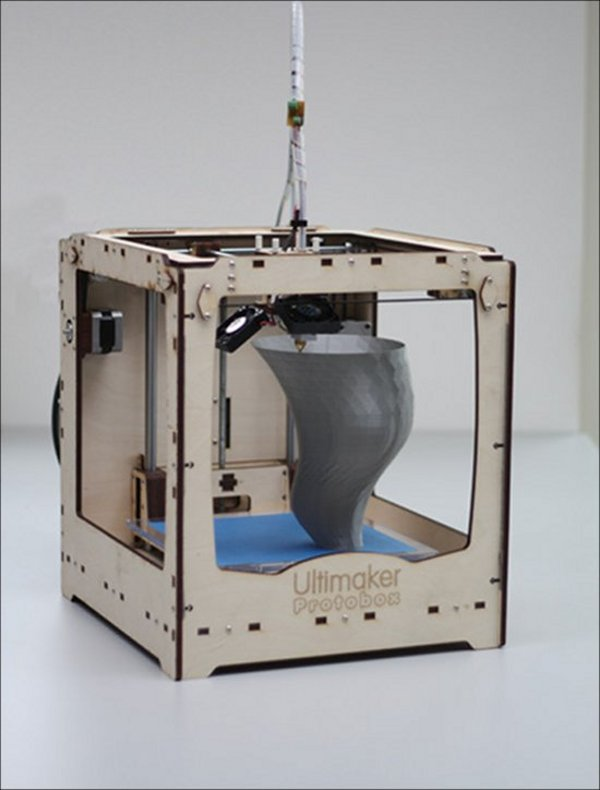
\includegraphics[width=4cm]{Ultimaker}	
		\end{figure}
  	\end{column}
  
  	\begin{column}{5cm}
  		\begin{block}{Process description}
  		\begin{enumerate}
  		\item The mesh is sliced to create instructions
  		\item The instructions are sent to the printer
  		\item The object is created by laying down successive layers of material
  		\end{enumerate}
 	 	\end{block}   
  	\end{column}
 	\end{columns}  
\end{frame}


\subsection{Objectives}
\begin{frame}
	\frametitle{The main client's requests}
	\begin{block}{Main goals of the project} 
	\begin{itemize}
		\item open-source modeler able to import, model, deform and \textbf{correct} virtual 3D objects
		\item interactions using the touchscreen
		\item export meshes to the printer
		\item print as realistically as possible
	\end{itemize}
    \end{block}
    
    \begin{block}{The final users}
    	\begin{itemize}
		\item The VORTEX team
		\item Some artists from Artilect for example (or artists students)
		\end{itemize}
    \end{block}
    
\end{frame}

\section{Project management}

\begin{frame}
	\frametitle{The tools}
	\begin{block}{}
    \begin{itemize}
		\item a web based project management system : Chiliproject (Gantt charts, calendars, documents, wiki, notifications\ldots )
		\item code management with Git
		\item an industrial supervisor from Airbus : Lionel Cremel
		\item weekly meetings with the supervisor, less often with clients
	\end{itemize}
	\end{block}
\end{frame}

\begin{frame}
	\frametitle{The V cycle management strategy}
	\begin{center}
		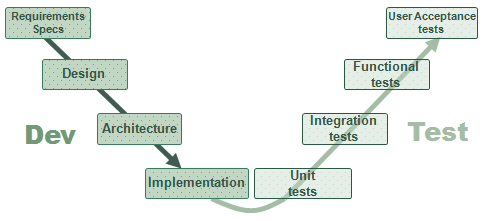
\includegraphics[width=\textwidth]{VCycle}	
	\end{center}
    
\end{frame}

\begin{frame}
	\frametitle{The macroscopic planning}

    \begin{center}
		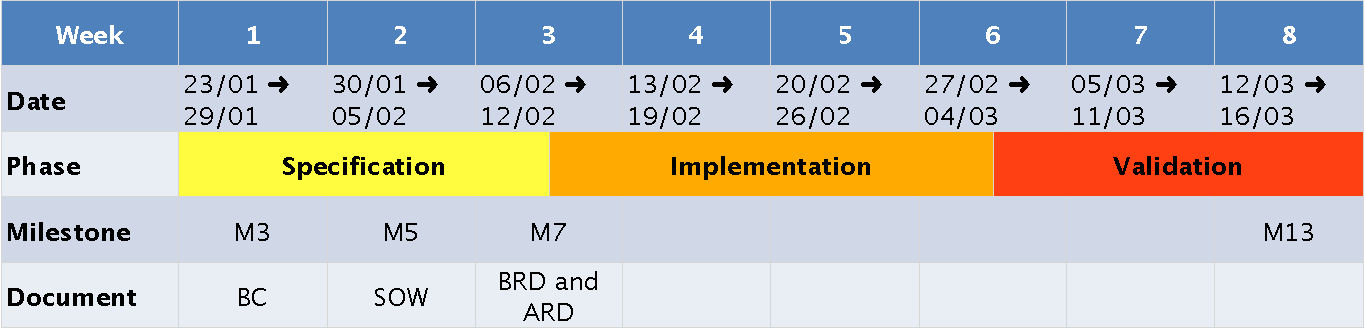
\includegraphics[width=\textwidth]{planning}	
	\end{center}
	
	\begin{block}{}
    \begin{itemize}
		\item Mx: milestones to respect: mainly documents to provide
		\item BC: Business Case
		\item SOW: Statement Of Work
		\item BRD \& ARD: the application design 
	\end{itemize}
	\end{block}
	
\end{frame}


\section{Architecture of the project}

\begin{frame}
	\frametitle{A four steps application}
	
	\begin{block}{}
		\begin{itemize}
			\item Modeler: to import/create STL and PLY meshes and to pre-process them
			\item G-code generator: to generate printing instructions
			\item Printer's driver: to send the instructions including special parameters such as the temperature
			\item Printer: to create the final object
		\end{itemize}
	\end{block}
	
\end{frame}


\begin{frame}
	\frametitle{From the modeler to the printer…}

    \begin{center}
		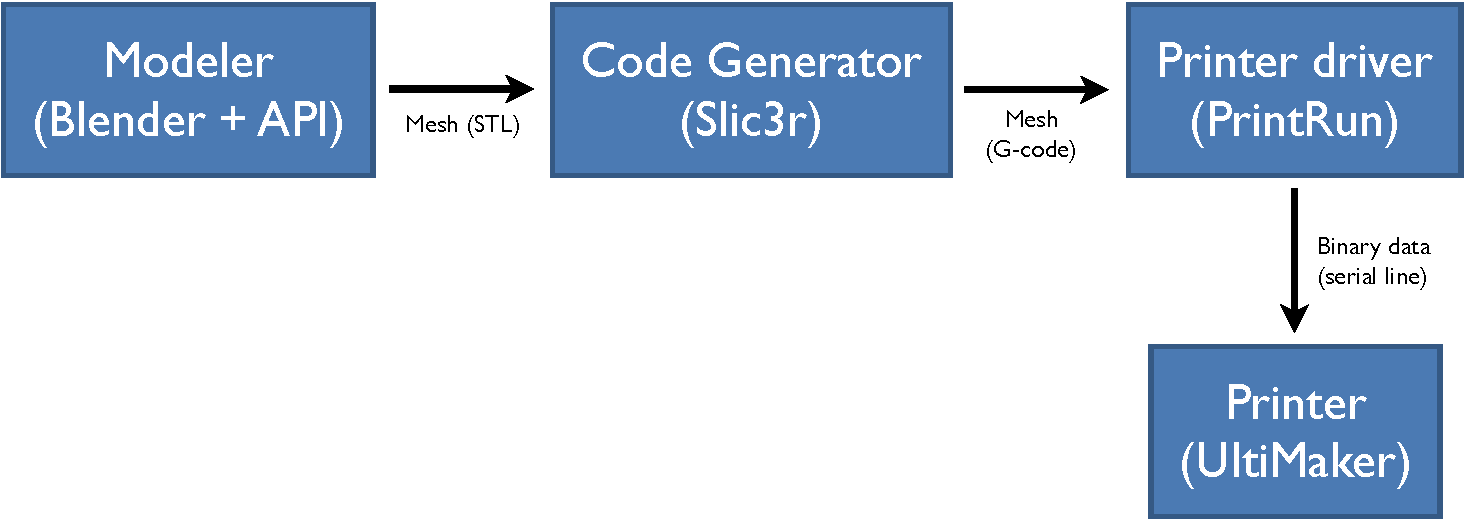
\includegraphics[width=10cm]{schema}	
	\end{center}
	
\end{frame}

\section{The main specifications}

\subsection{About the global application}
\begin{frame}
	\frametitle{}
	 \begin{block}{The application characteristics}
		\begin{itemize}
			\item must be fully open source
			\item must be usable on both Linux Ubuntu and Windows (if possible)
			\item must be delivered as an archive
		\end{itemize}
    \end{block}
\end{frame}
    
\subsection{About the modeler}
\begin{frame}
	\frametitle{}
	 \begin{block}{The modeler characteristics}
		\begin{itemize}
			\item must allow the import of STL and PLY meshes
			\item must allow the export of STL meshes
			\item all the functions implemented must be run in less than a few hours
		\end{itemize}
    \end{block}
    
    \begin{block}{The interactions required on the meshes}
		\begin{itemize}
			\item 
			\item 
		\end{itemize}
    \end{block}

\end{frame}

\subsection{About the documentation}
\begin{frame}
	\frametitle{}
	 \begin{block}{The documentation required}
		\begin{itemize}
			\item a user documentation: to use the application properly just by reading it. It should include the limits of the application.
			\item a technical documentation: so that the client or an other team can continue the work if needed
			\item an installation paper: to enable the user to get an operational application from the initial archive
		\end{itemize}
    \end{block}    

\end{frame}

\section{Our technical solutions and results}

\subsection{Choice of the modeler}
\begin{frame}
	\frametitle{}
		--> Implementation of a modeler from scratch excluded \\
		--> Choice reduced to Blender or Meshlab
    \begin{columns}[t]
  	\begin{column}{5cm}
  		\begin{block}{Meshlab}
  		Advantages:
  		\begin{itemize}
  		\item very light application
  		\item preexisting functions for mesh correction
  		\end{itemize}
  		
  		Drawbacks:
  		\begin{itemize}
  		\item no integrated interaction
  		\end{itemize}
 	 	\end{block}   
  	\end{column}
  
  	\begin{column}{5cm}
  		\begin{block}{Blender (the chosen one)}
  		Advantages:
  		\begin{itemize}
  		\item interactions preexisting 
  		\item Python API  
  		\item a lot of documentation
  		\item manually modifiable GUI
  		\end{itemize}
  		
  		Drawbacks:
  		\begin{itemize}
  		\item many useless things
  		\end{itemize}
 	 	\end{block}   
  	\end{column}
 	\end{columns}  
    
\end{frame}

\subsection{Mesh correction integration}
\begin{frame}
	\frametitle{}

    \begin{block}{Manifold correction}
		\begin{itemize}
			\item manifold checking and hole filling already included in Blender
			\item some bad results
			\item parler du temps d'execution et des limites
		\end{itemize}
    \end{block}
    
    \begin{block}{Choice of the orientation}
		\begin{itemize}
			\item parler du temps d'execution et des limites
		\end{itemize}
    \end{block}
    
\end{frame}

\subsection{Modifications in Blender's interface}
\begin{frame}
	\frametitle{}

    \begin{block}{A new screen for Blender}
Possibility in Blender to manually modify the interface and to register it as the default one.
Changes operated:
    \end{block}
    
    \begin{block}{A new panel}
    \begin{itemize}
	\item Addition on a new panel named "Mesh verification" thank to the Blender Python API
	\item Insertion of buttons appearing conditionally and calling the mesh corrections implemented
	\end{itemize}
    \end{block}
    
    \begin{block}{Progression bar integration}

    \end{block}
    
\end{frame}

\subsection{Calibration of the printer}
\begin{frame}
	\frametitle{}

    \begin{block}{The choice of the parameters}
    \end{block}
\end{frame}

\section{Conclusions and thanks}
\begin{frame}
	\frametitle{}

    \begin{block}{}
    \end{block}
\end{frame}

\begin{frame}
	\frametitle{}

    \begin{center}
    \Large{Thank you for your attention !}
    \end{center}
\end{frame}
	
\end{document}
